\documentclass[a4paper, 12pt]{article}
\usepackage{graphicx}
\usepackage{url}
\usepackage{hyperref}
\usepackage[numbers]{natbib}
\usepackage{tabularx}
\usepackage{amsmath}
\usepackage{amssymb}
\usepackage{epstopdf}
\usepackage{inputenc}
\usepackage{geometry}
\usepackage{alphabeta}
\usepackage{float}
\usepackage{changepage}
\usepackage{lipsum}

\setlength{\oddsidemargin}{0mm}
\setlength{\evensidemargin}{-14mm}
\setlength{\marginparwidth}{0cm}
\setlength{\marginparsep}{0cm}
\setlength{\topmargin}{2mm}
\setlength{\headheight}{0mm}
\setlength{\headsep}{0cm}
\setlength{\textheight}{240mm}
\setlength{\textwidth}{168mm}
\setlength{\topskip}{0mm}
\setlength{\footskip}{10mm} 

\newcommand{\code}[1]{\texttt{#1}}
\newcommand{\refsec}[1]{\mbox{Section~\ref{sec:#1}}}
\newcommand{\refapp}[1]{\mbox{Appendix~\ref{sec:#1}}}
\newcommand{\refeqn}[1]{\mbox{(\ref{eqn:#1})}}
\newcommand{\reffig}[1]{\mbox{Figure~\ref{fig:#1}}}
\newcommand{\ud}{\mathrm{d}}                    % upright d (derivative)

\newcounter{foo}
\newcounter{bar}

\title{
    ENEL420 - Genetic Algorithms in Digital Signal Processing\\
    \vspace{1cm}
    \begin{large} 
        Department of Electrical and Computer Engineering\\
        University of Canterbury\\
    \end{large}
    \vspace{1cm}
}

\author{
    \small {Luke Trenberth (ID: 47277086)}\\
    \small {Hassan Alhujhoj (ID: 35352633)}\\
    }
\vspace{2cm}

\date{\small\today}
\begin{document}
\maketitle

\begin{abstract}
    I would like to say some bullshit here that summaries my report in an interesting way.
\end{abstract}

\pagebreak
\pagenumbering{roman}
\tableofcontents
\pagenumbering{arabic}
\pagebreak

\section{Introduction}\label{sec:intro}
    Introduction\cite{Ifeachor1995}.Plz write something here.

\section{Background}\label{sec:bg}
    \subsection{Digital Signal Processing of ECG Signals}\label{sec:bg_sub1}
        In assignment one, a noisy ECG signal with 1024Hz sampling frequency was provided to be filtered. 
        The assignment required the implementation of a notch filter with either an FIR or IIR filter.
        An FIR or IIR notch filter was suited to filter this ECG signal since there were a clear two 
        interference frequencies present within the frequency spectrum of the ECG signal.
        These interference frequencies were identified to be $f_{1} = 31.456Hz$ and $f_{2} = 74.36Hz$
        as shown in Figure \ref{Fig:fig1}. It should be noted that the first peak in Figure \ref{Fig:fig1} is the 
        DC component due to the use FFT to get the frequency response of the time domain ECG signal.
        
        \begin{figure}[h!]
            \centering
            \graphicspath{{./wiki/}}
            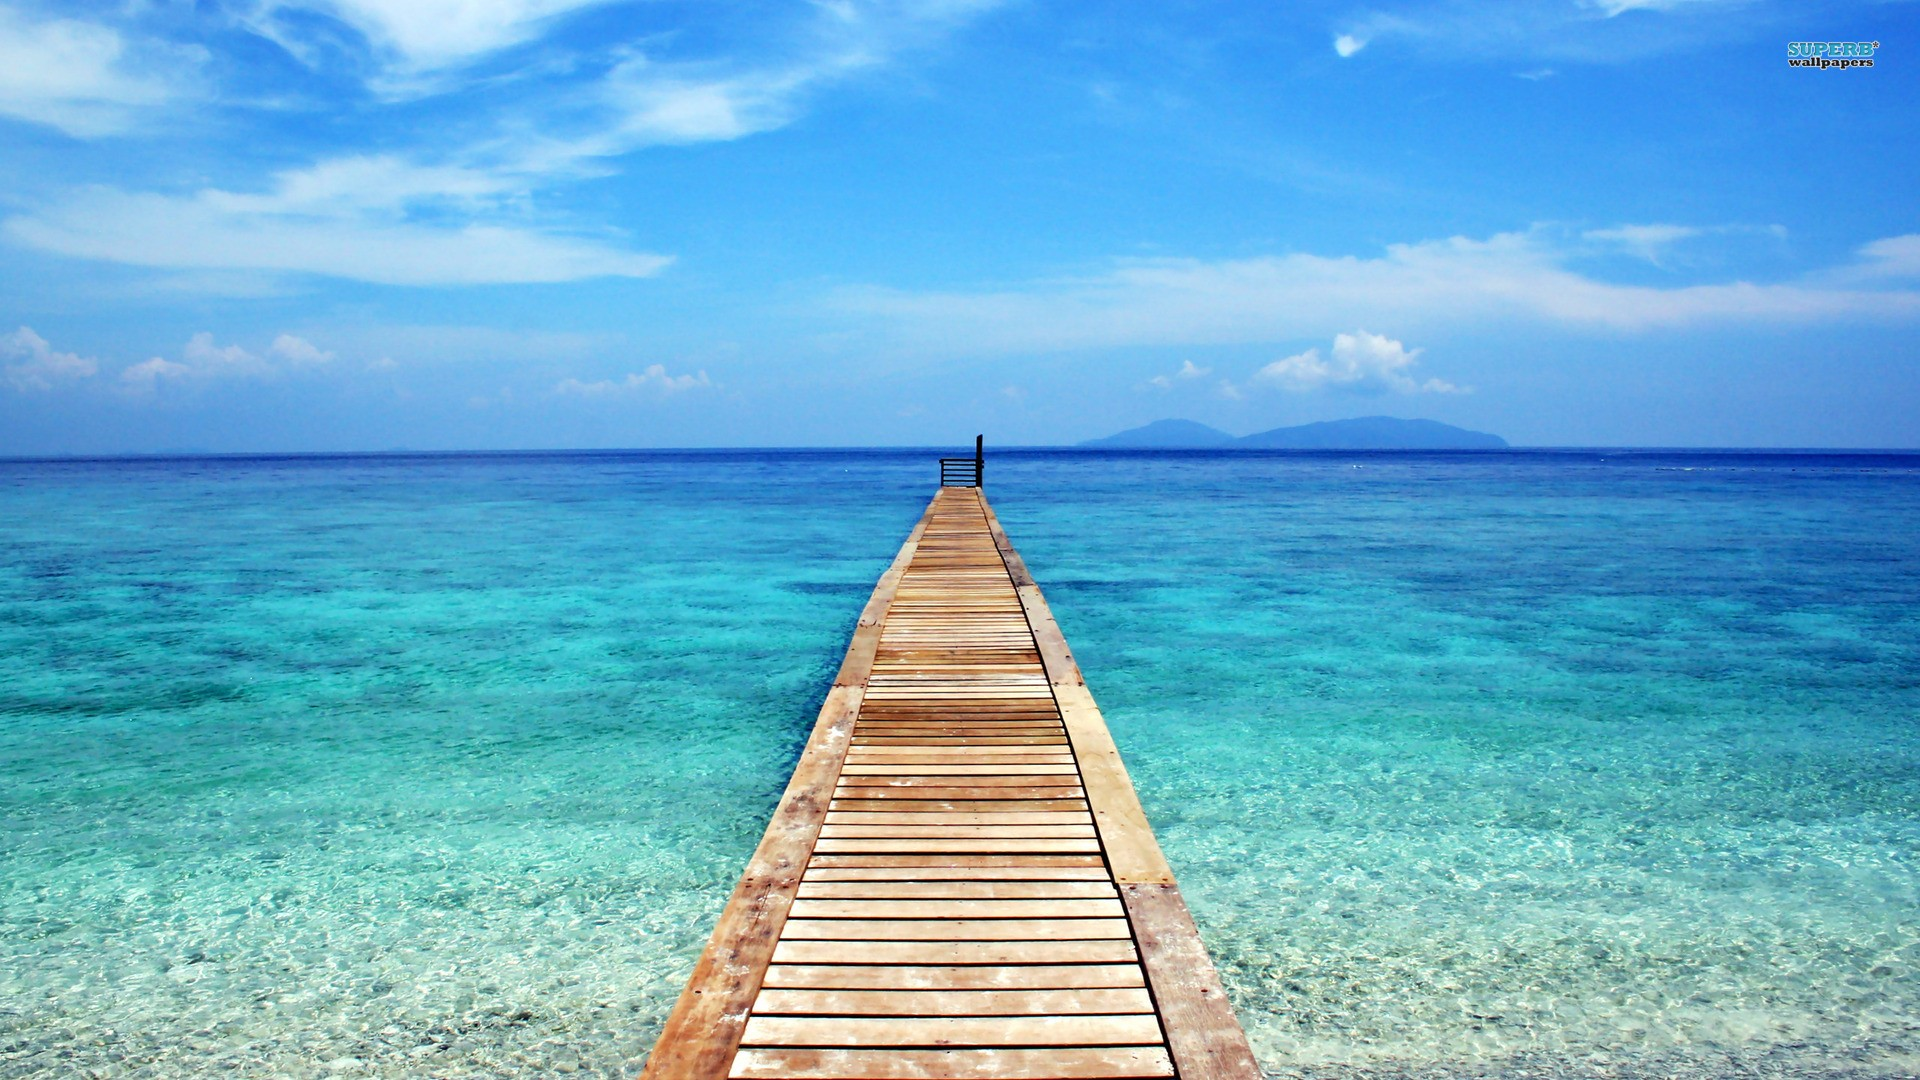
\includegraphics[scale=0.6]{fig1.png}
            \caption{Interference frequencies present in the ECG signal.}
            \label{Fig:fig1}
        \end{figure}

        One method to filter these two frequencies was to reject them with a 2-pole cascaded IIR notch filter
        
    \subsection{Genetic Algorithms}\label{sec:bg_sub2}
        Plz write something here.

\section{Method}\label{sec:meth}
    Describe the method followed for this assignment.
    \subsection{Creating a Population from DSP Singal Data}\label{sec:meth_sub1}
        Plz write something here.
    \subsection{Fitness Function}\label{sec:meth_sub2}
        Plz write something here.
    \subsection{Selecting Paranets for next GA Generations}\label{sec:meth_sub3}
        Plz write something here.
    \subsection{GA Operators}\label{sec:meth_sub4}
        Plz write something here.
        \subsubsection{Crossover}
            Plz write something here.
        \subsubsection{Mutation}
            Plz write something here.
        \subsubsection{Parents}
            Plz write something here.
    \subsection{Filtering of ECG Signal Using FIR Filters}\label{sec:meth_sub5}
        \subsubsection{Window Filter}
            Plz write something here.
        \subsubsection{Parks-McClellan Filter}
            Plz write something here.
    
    \begin{flushleft}
        ex1\\
        ex2\\
        ex3\\
        1 format1\\
        2 foramat2\\
    \end{flushleft}

\section{Results}\label{sec:res}
    Describe\ae the results you've got. Don't give your opinion in here that goes in the Discussion.
    Unless combine the Results and Discussion sections \begin{equation} V = IR\end{equation}.

    \begin{list}{S-\arabic{foo}}{\usecounter{foo}}
        \item item1.
        
        \item item2.
        
        \item item3.
    \end{list}

    \begin{figure}[h]
        \centering
        \graphicspath{{./wiki/}}
        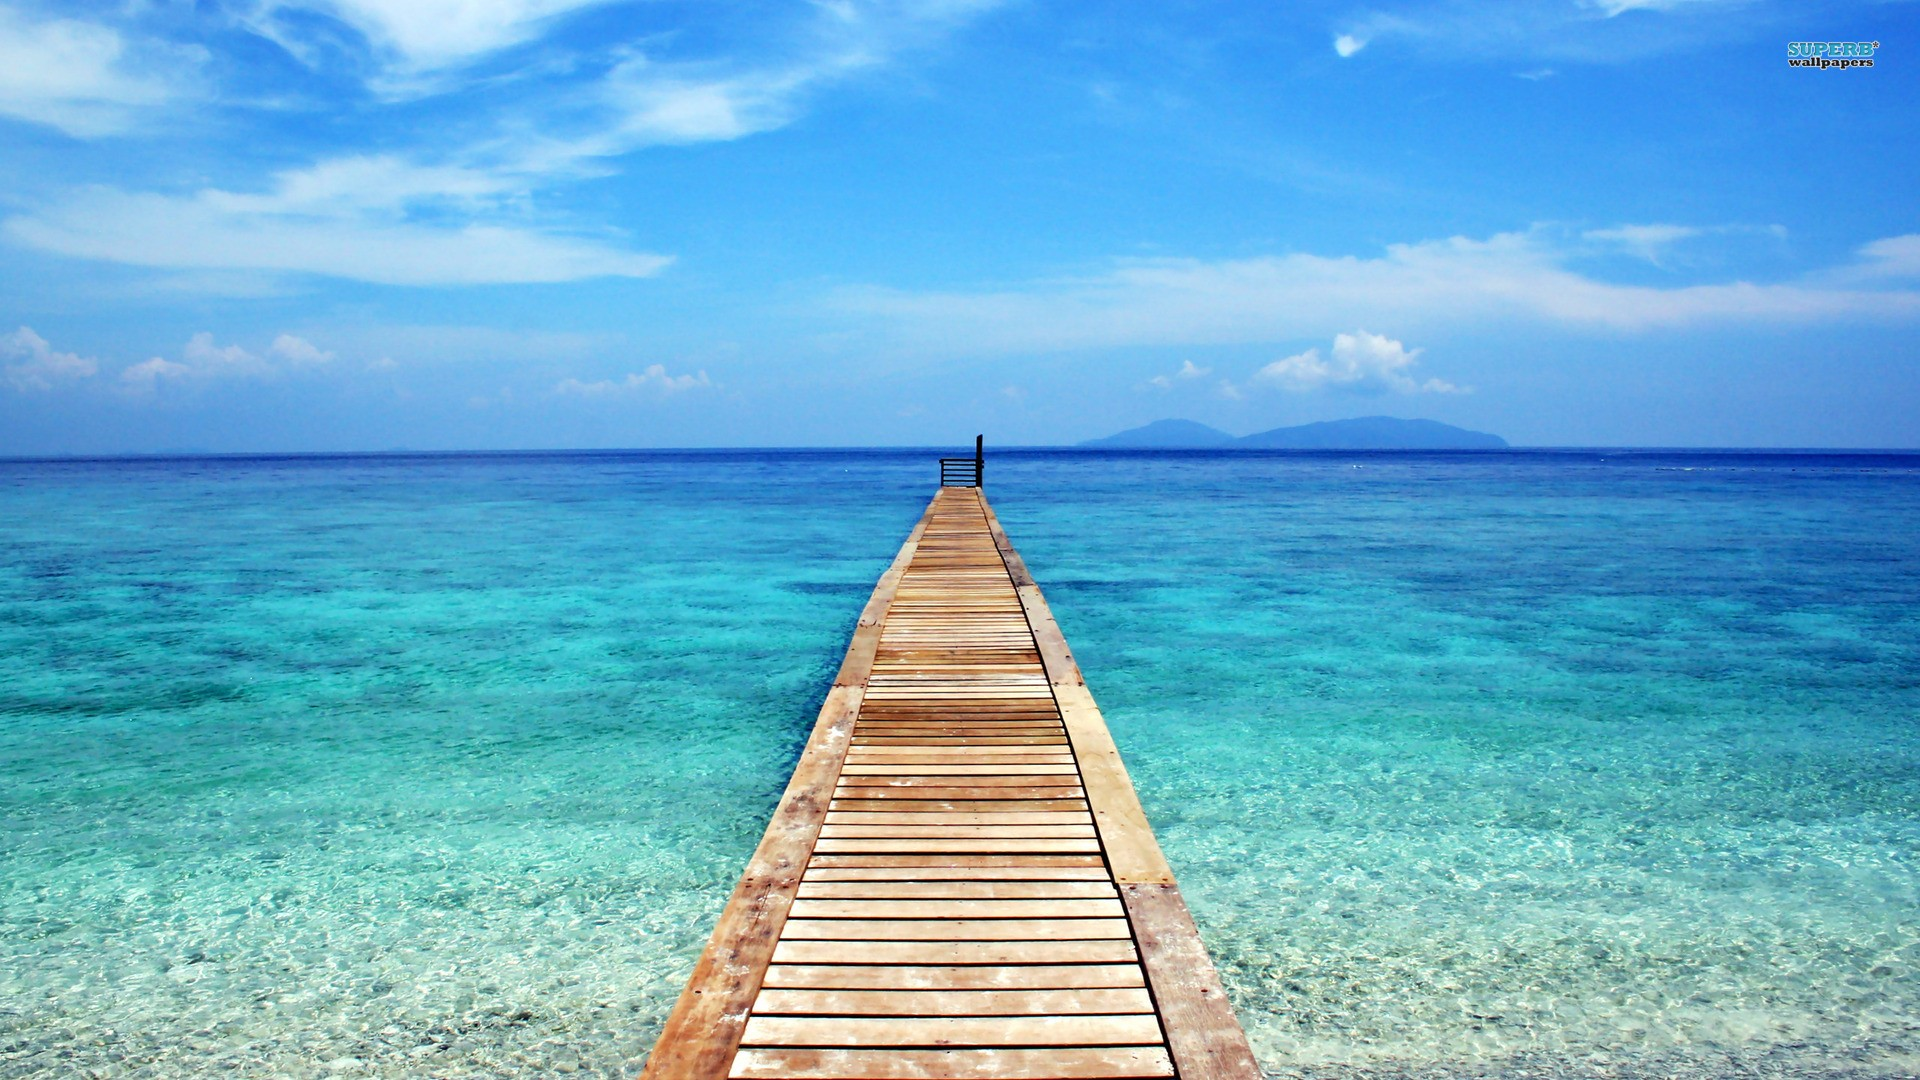
\includegraphics[scale=0.1]{fig.png}
        \caption{Shows that you can relax at this beautiful beach}
        \label{Fig:my_label}
    \end{figure}

\section{Discussion}\label{sec:dis}
    Discussion.

\section{Conclusion}\label{sec:conc}
    Reinstate the stuff you've talked about in the report. Don't introduce new materials in here.

\pagebreak
\bibliographystyle{IEEEtran}
\renewcommand{\bibname}{References}
\renewcommand{\bibsection}{\section{\bibname}}
\renewcommand{\cite}{\citep}
\bibliography{ref}
\pagebreak

\section{Appendices}
    \subsection{Appendix A}

\end{document}

